\DiaryEntry{Poisson Process, 1}{2019-01-07}{Stochastic}

Based on \href{https://ocw.mit.edu/courses/electrical-engineering-and-computer-science/6-262-discrete-stochastic-processes-spring-2011/course-notes/MIT6_262S11_chap02.pdf}{these notes.}

\subsection{Arrival Process}

An arrival process is a sequence of increasing RVs, $0 < S_1 < S_2 < \cdots$, where the $S_i$ are called arrival times or arrival epochs. They could be interpreted as the times some repeating phenomenon occurs. The process starts at time $0$ and note that events cannot happen at the same time (since the $S_is$ are distinct values).

In order to describe the arrival process, the joint pdf of the $S_i$s must be known.

There are two additional description methods: The first one is via the interarrival times $X_i = S_i - S_{i-1}$ (with the special case $X_1 = S_1$); the arrival times can be obtained via

\be\label{2019-01-07_eq0}
S_n = \sum_{i=1}^n X_i
\ee

The joint distribution of the $X_i$s is sufficient and typically easier to obtain as the interarrival times are usually iid.

The second description method is the counting process $\{N(t); t>0\}$ where $N(t)$ counts the number of arrivals between $0$ and up to (and including) $t$ (i.e. in the interval $(0,t]$). In other words, $N(t) = n$ for $S_n \leq n \leq S_{n+1}$. $N(0)$ is defined as $N(0) = 0$ and we have $N(t) \geq N(\tau)$ for $t \geq \tau > 0$.

The whole story is best explained via the following Figure

\begin{figure}[H]
  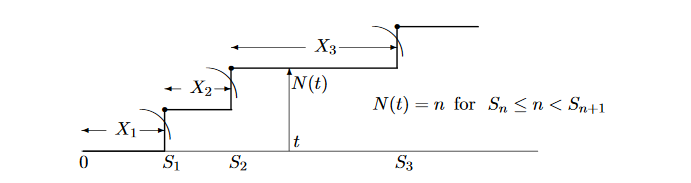
\includegraphics[scale=0.8]{images/poisson_process_1_1.png}
\end{figure}

The counting process and the arrival times are related according to

\be\label{2019-01-07:eq1}
\{S_n \leq t\} = \{N(t) \geq n\}
\ee

This can be understood as follows: For a fixed point in time $t$ (see Figure above), if the event $S_n \leq t$ has happened, then $N(t)$ must be $\geq n$.

Conversely, we have

\bee
\{S_n > t\} = \{N(t) < n\};
\eee

i.e. when the event $S_n > t$ (for a fixed time $t$), then $N(t)$ must be $< n$. 

\subsection{Poisson Process}

We have the following two definitions:

\begin{definition}[Renewal Process]
  A renewal process is an arrival process for which the sequence of interarrival times is a sequence of iid RVs.
\end{definition}


\begin{definition}[Poisson Process]

  A Poisson Process is a renewal process in which the interarrival times have an exponential distribution; i.e. each $X_i$ has the pdf

  \bee
    f_X(x) = \lambda e^{-\lambda x}, \quad \lambda > 0
  \eee
  
\end{definition}

The Poisson process is unique among renewal processes in that its interarrival times are  memoryless.

\begin{definition}[Memoryless RVs]
A positive RV $X$ is called memoryless, if it has the following property ($x,t \geq 0$)

\bee
P(X_i > t+x) = P(X_i > t) P(X_i > x)
\eee

where $\lambda$ denotes the rate of the process.

\end{definition}

For an exponential distribution, we have

\bee
P(X>t) = \int_t^\infty \lambda e^{-\lambda x} dx = e^{-\lambda t}
\eee

and therefore

\bee
P(X > t+x) = e^{-\lambda (t+x)} = e^{-\lambda t} e^{- \lambda x} = P(X > t)P(X > x) \qed
\eee

The exponential distribution is the only continuous distribution having the memoryless property. From the memorylessness follows

\begin{align*}
P(X>t+x|X>t) = \frac{P(X>t+x, X>t)}{P(X>t} = \frac{P(X>t+x)}{P(X>t} &= \frac{P(X>t)P(X>x)}{P(X>t)} \\ &= P(X>x)
\end{align*}

This can be interpreted as follows: If an event has not occured until time $t$, the distribution of the remaining waiting time $x$ is the same as the distribution of the original waiting time; i.e. the remaining waiting time has no memory of the previous waiting.

\subsection{Further Results}

\paragraph{Distribution of $S_n$.} The $n$-th arrival time $S_n$ is given as sum of $n$ RVs each having exponential distribution. The pdf of $S_n$ is then the $n$-fold convolution of these exponential distributions which can be shown to be the Erlang distribution

\bee
f_{S_n}(t) = \frac{\lambda^n t^{n-1}e^{-\lambda t}}{(n-1)!}
\eee

The mean can be calculated as follows

\bee
E\{S_n\} = \int \frac{\lambda^n t^{n}e^{-\lambda t}}{(n-1)!} dt = \frac{\lambda^n}{(n-1)!} \int t^{n}e^{-\lambda t} dt
\eee

With a small substitution the integral can be solved by the Gamma function: $u=\lambda t \rightarrow t=u/\lambda, dt = du/\lambda$ and we have

\bee
E\{S_n\} = \frac{\lambda^n}{(n-1)!} \frac{1}{\lambda} \int \left(\frac{u}{\lambda}\right)^n e^{-u} du = \frac{1}{\lambda (n-1)!} \Gamma(n+1) = \frac{1}{\lambda (n-1)!} n! = \frac{n}{\lambda}
\eee

This can be interpreted that every event contributes $1/\lambda$ to the mean of $S_n$. \qed

The maximum of the distribution (the mode), $t^\star$, can be obtained by setting the derivative (wrt $t$) to zero. The derivative is

\bee
\frac{d f_{S_n}(t)}{dt} \propto (n-1) t^{n-2}e^{-\lambda t} - \lambda t^{n-1}e^{-\lambda t}
\eee

Setting it to zero yields for the mode

\bee
t^\star = \frac{n-1}{\lambda} \qed
\eee

\paragraph{Proof of Erlang distribution.} The distribution of $S_2$ is given by
\bee
f_{S_2}(x) = \int f_{X_1}(t) f_{X_2} (x-t) dt = \int \lambda e^{-\lambda t} \lambda e^{-\lambda (x-t)} dt = \lambda^2 \int e^{-\lambda x}dt \propto t e^{-\lambda t}
\eee

Interestingly, the $e^{\lambda t}$ terms cancel, leaving something constant (in $t$). Integrating this over $t$, yields the constant times something proportional in $t$. The distribution of $S_3$ can be obtained similarly,

\bee
f_{S_3}(x) = \int f_{X_1}(t) f_{S_2} (x-t) dt \propto \int \lambda e^{-\lambda t} (x-t) e^{-\lambda (x-t)} dt \propto t^2 e^{-\lambda t}
\eee

This (more or less) confirms that $S_n$ has an Erlang distribution. \qed

\paragraph{Distribution of $N(t)$.}

The PMF for $N(t)$ is the Poisson distribution

\bee
f_{N(t)}(n) = \frac{(\lambda t)^n e^{-\lambda t} }{ n!  }
\eee

The (probably) simpler proof is to start from the Poisson process definition, that $N(t)$ is Poisson distributed and show that the interarrival times have exponential distribution as consequence.

Let us start with the distribution of $X_1$. The probability that it happens after $t$ is given by

\bee
P(X_1 > t) = P(\text{no arrival in } (0,t]) = P(N(t) = 0) = \frac{(\lambda t)^0 e^{-\lambda t} }{ 0!  } = e^{-\lambda t} 
\eee

We continue with $X_2$: Assume the previous event $X_1$ happened at time $s$, we can calculate 
\bee
P(X_2 > t | X_1=s) = P(\text{no arrival in } (s,s+t] | X_1 = s) = P(\text{no arrival in } (s,s+t]) = e^{-\lambda s}
\eee

where we have used the memoryless property of the process and from which follows that $X_2$ also has exponential distribution. The generalization follows. \qed

The other approach is to start at \eqref{2019-01-07:eq1},

\bee
\{N(t) \geq n\} = \{S_n \leq t\}
\eee

and equate the probabilities of these two events

\bee
\sum_{i=n}^\infty p_{N(t)}(i) = \int_0^t f_{S_n}(\tau) d\tau
\eee

Inserting the Poisson distribution on the left, and taking the derivative on both sides, we obtain an Erlang distribution for $S_n$, which confirms that $N(t)$ follows a Poisson distribution. \qed

\subsection{Simulation Results}

In \href{}{this simulation}, we simulatea Poisson process by creating interarrival times with exponential distribution. By using \eqref{2019-01-07_eq0} we create the corresponding arrival times and finally count them in a window. Some care has to be taken that there are enough arrivals in the window by proper choice of parameters.


\begin{verbatim}
mean arrivals, simulation: 3.333635
mean arrivals, analytical result: 3.3333333333333335
k: 1 simulation: 0.118755 analytical result: 0.11891331115750799
k: 2 simulation: 0.198199 analytical result: 0.19818885192917998
k: 3 simulation: 0.220271 analytical result: 0.22020983547686668
k: 4 simulation: 0.183716 analytical result: 0.18350819623072223
k: 5 simulation: 0.122088 analytical result: 0.12233879748714817
k: 6 simulation: 0.068142 analytical result: 0.0679659986039712
k: 7 simulation: 0.032288 analytical result: 0.03236476123998628
k: 8 simulation: 0.013467 analytical result: 0.013485317183327622
k: 9 simulation: 0.005091 analytical result: 0.004994561919750971
k: 10 simulation: 0.001654 analytical result: 0.0016648539732503236
\end{verbatim}


%%% Local Variables:
%%% mode: latex
%%% TeX-master: "journal"
%%% End:
